\begin{figure}[ht]
	\centering 
	\begin{subfigure}[t]{1\linewidth} \centering
		\makebox[0.15\linewidth]{}
		\makebox[0.180\linewidth]{\textbf{Car}}
		\makebox[0.180\linewidth]{\textbf{Bearing}}
		\makebox[0.180\linewidth]{\textbf{Knob}}
		\makebox[0.180\linewidth]{\textbf{Bracket}}
	\end{subfigure}
	\begin{subfigure}[t]{1\linewidth} \centering
		\phantomcaption 
		\label{fig/eval/mvs/input}
		\makebox[0.15\linewidth]{\raisebox{0.07\linewidth}{(a) Input}}		
		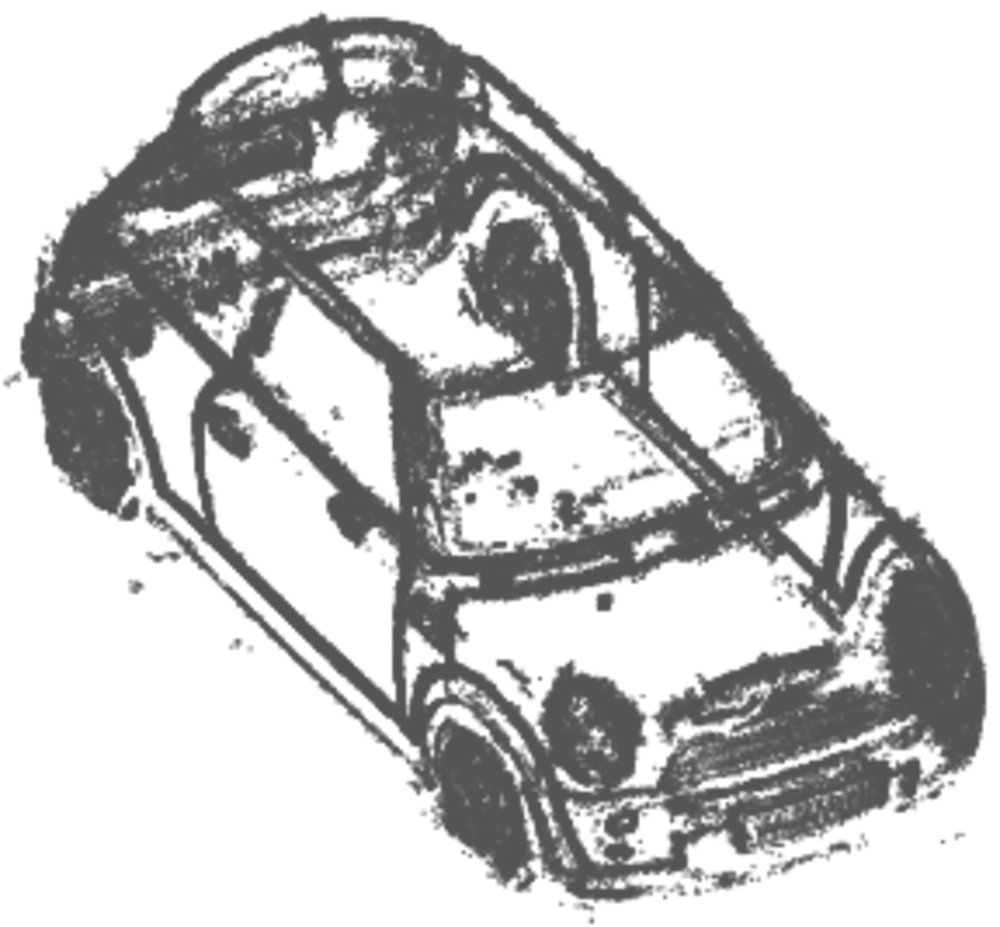
\includegraphics[width=0.180\linewidth]{./fig/eval/mini_input.jpg}
		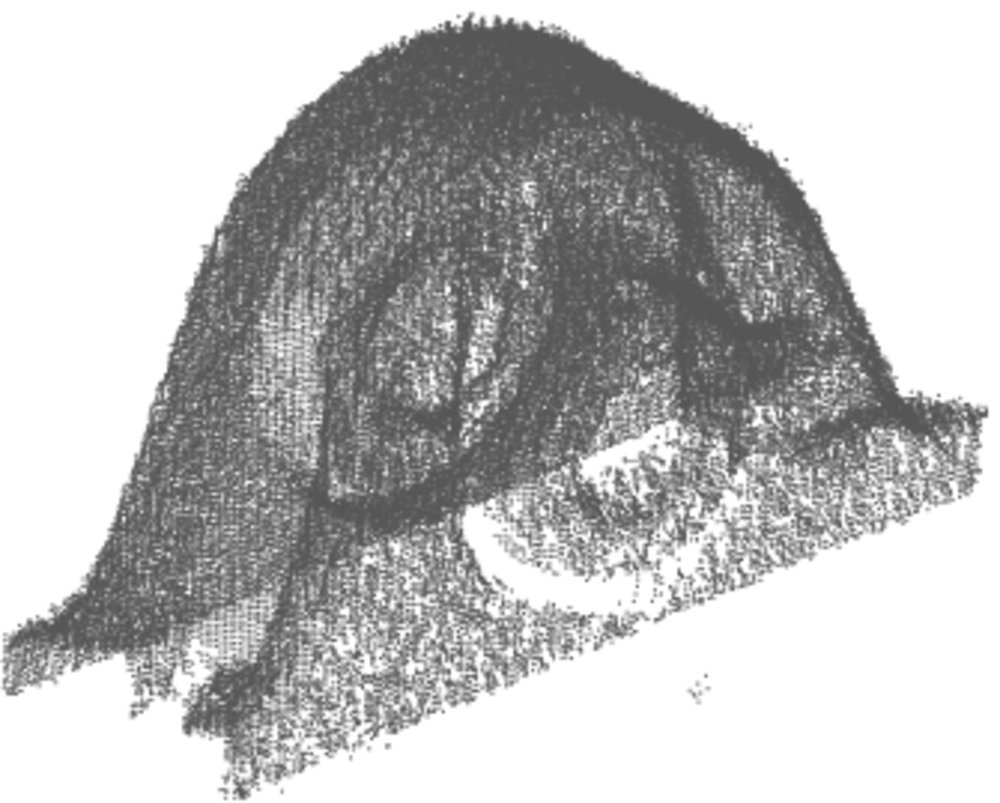
\includegraphics[width=0.180\linewidth]{./fig/eval/bearing_input.jpg} 
		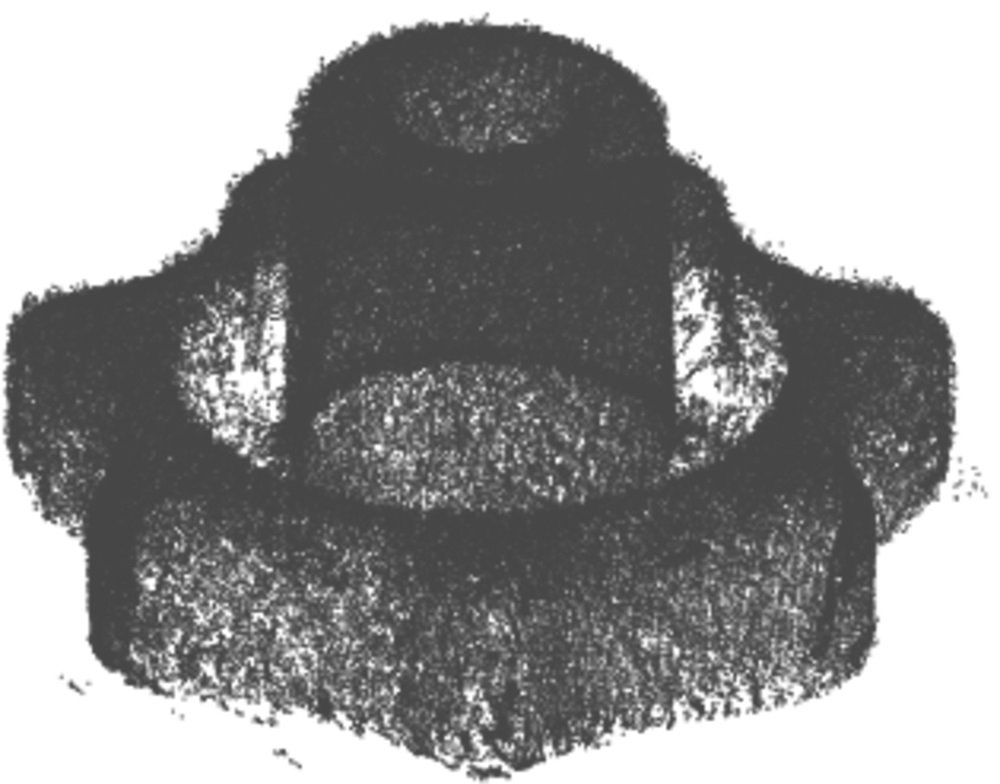
\includegraphics[width=0.180\linewidth]{./fig/eval/knob_input.jpg} 
		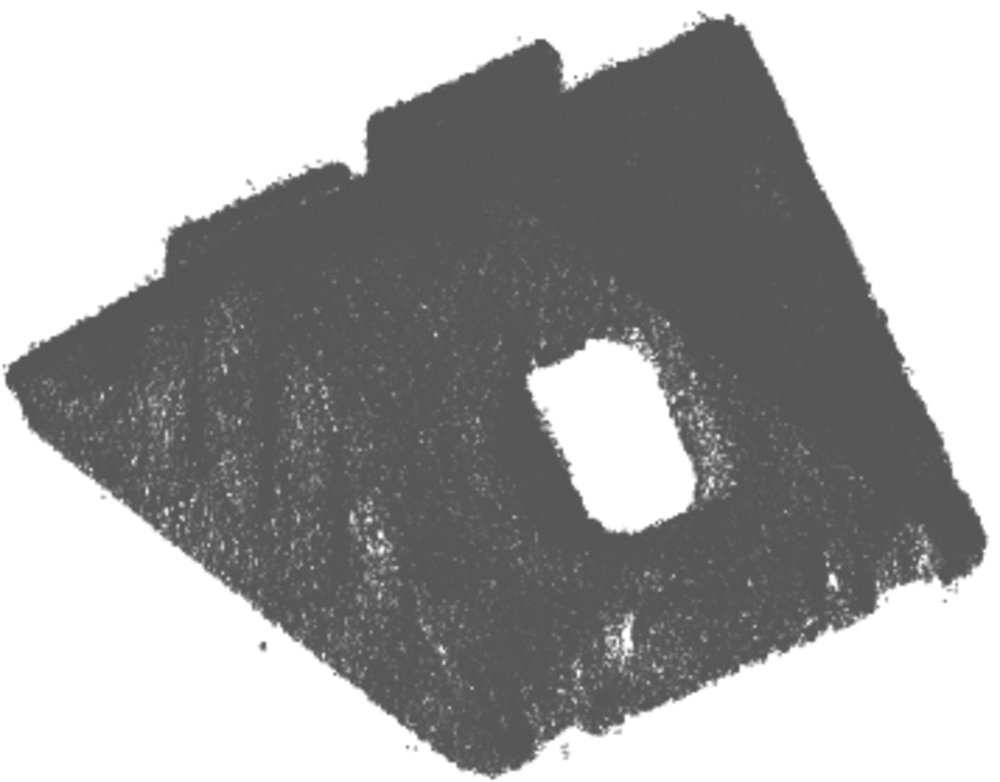
\includegraphics[width=0.180\linewidth]{./fig/eval/bracket_input.jpg} 
	\end{subfigure}
	\begin{subfigure}[t]{1\linewidth} \centering
		\phantomcaption 
		\label{fig/eval/mvs/dog}
		\makebox[0.15\linewidth]{\raisebox{0.07\linewidth}{(b) DoG}} 
		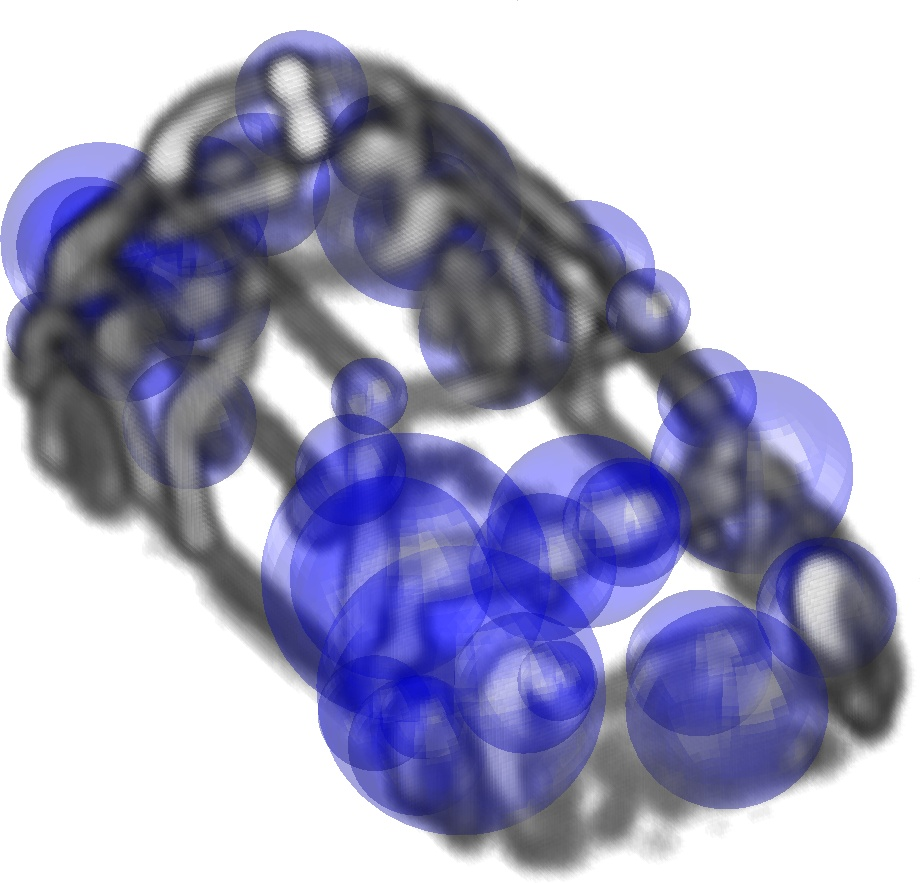
\includegraphics[width=0.180\linewidth]{./fig/eval/mini_dog.jpg} 
		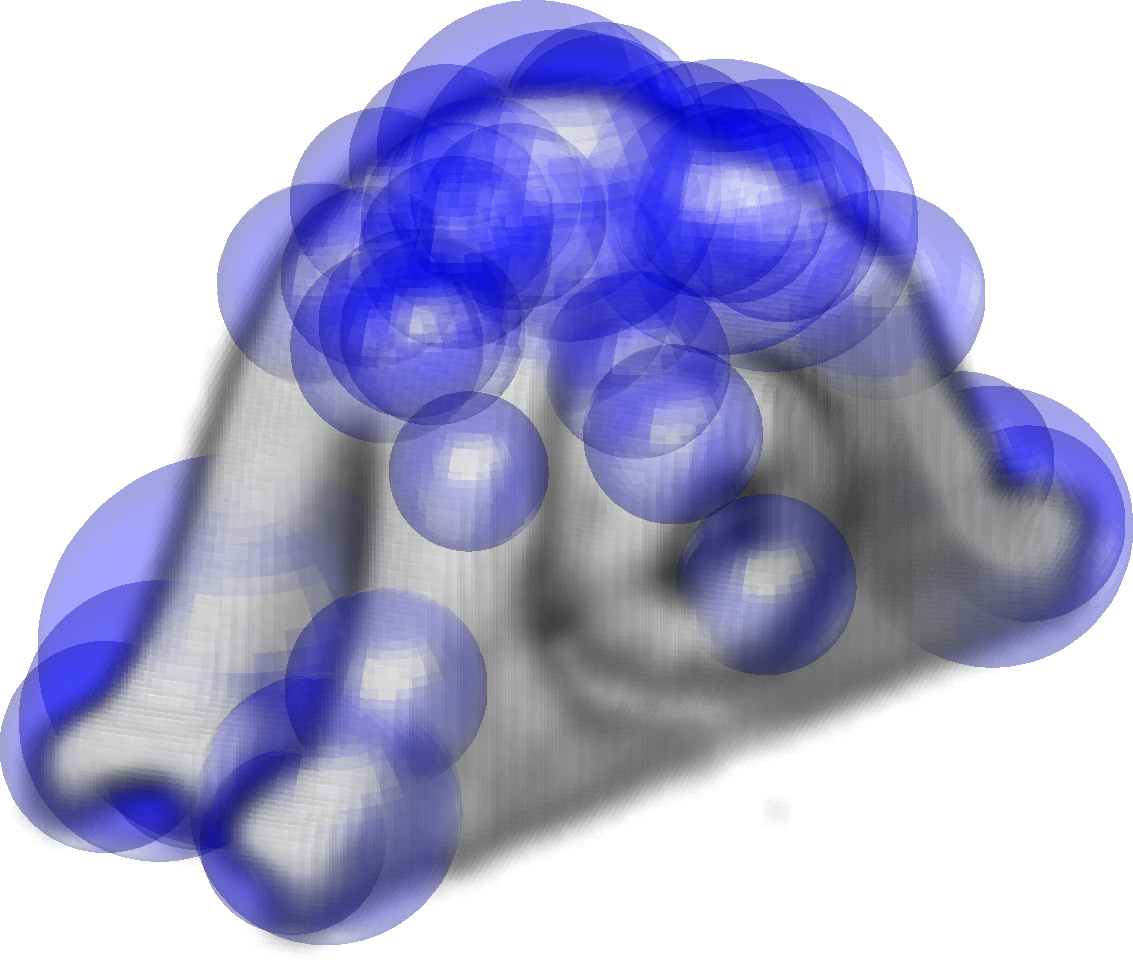
\includegraphics[width=0.180\linewidth]{./fig/eval/bearing_dog.jpg}  
		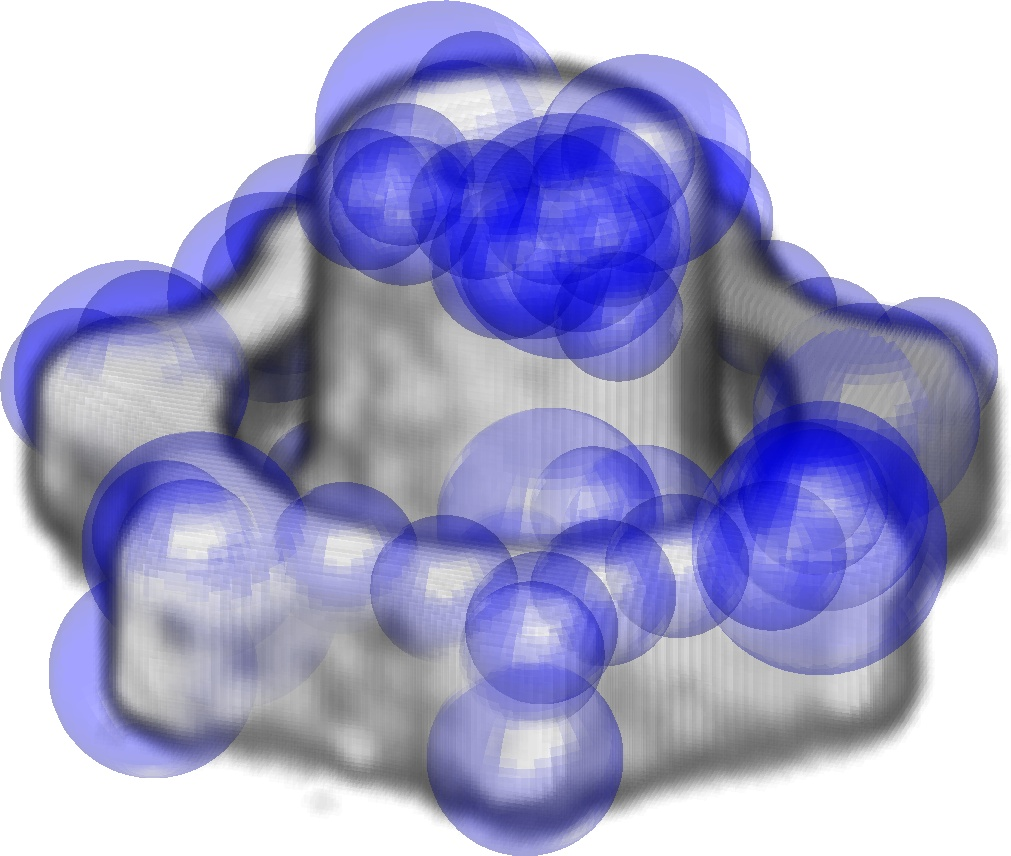
\includegraphics[width=0.180\linewidth]{./fig/eval/knob_dog.jpg} 
		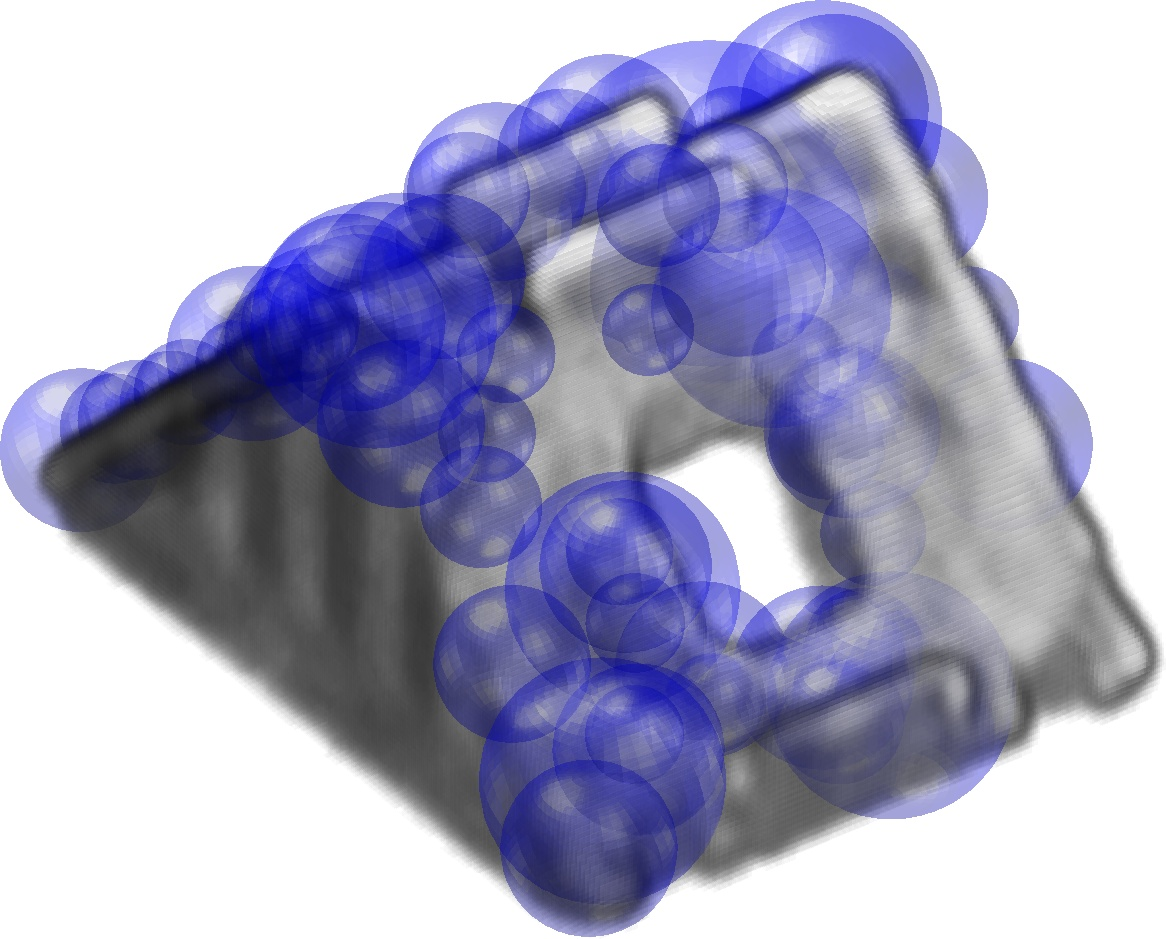
\includegraphics[width=0.180\linewidth]{./fig/eval/bracket_dog.jpg} 
	\end{subfigure}
	\begin{subfigure}[t]{1\linewidth} \centering
		\phantomcaption 
		\label{fig/eval/mvs/surf}
		\makebox[0.15\linewidth]{\raisebox{0.07\linewidth}{(c) SURF}}		
		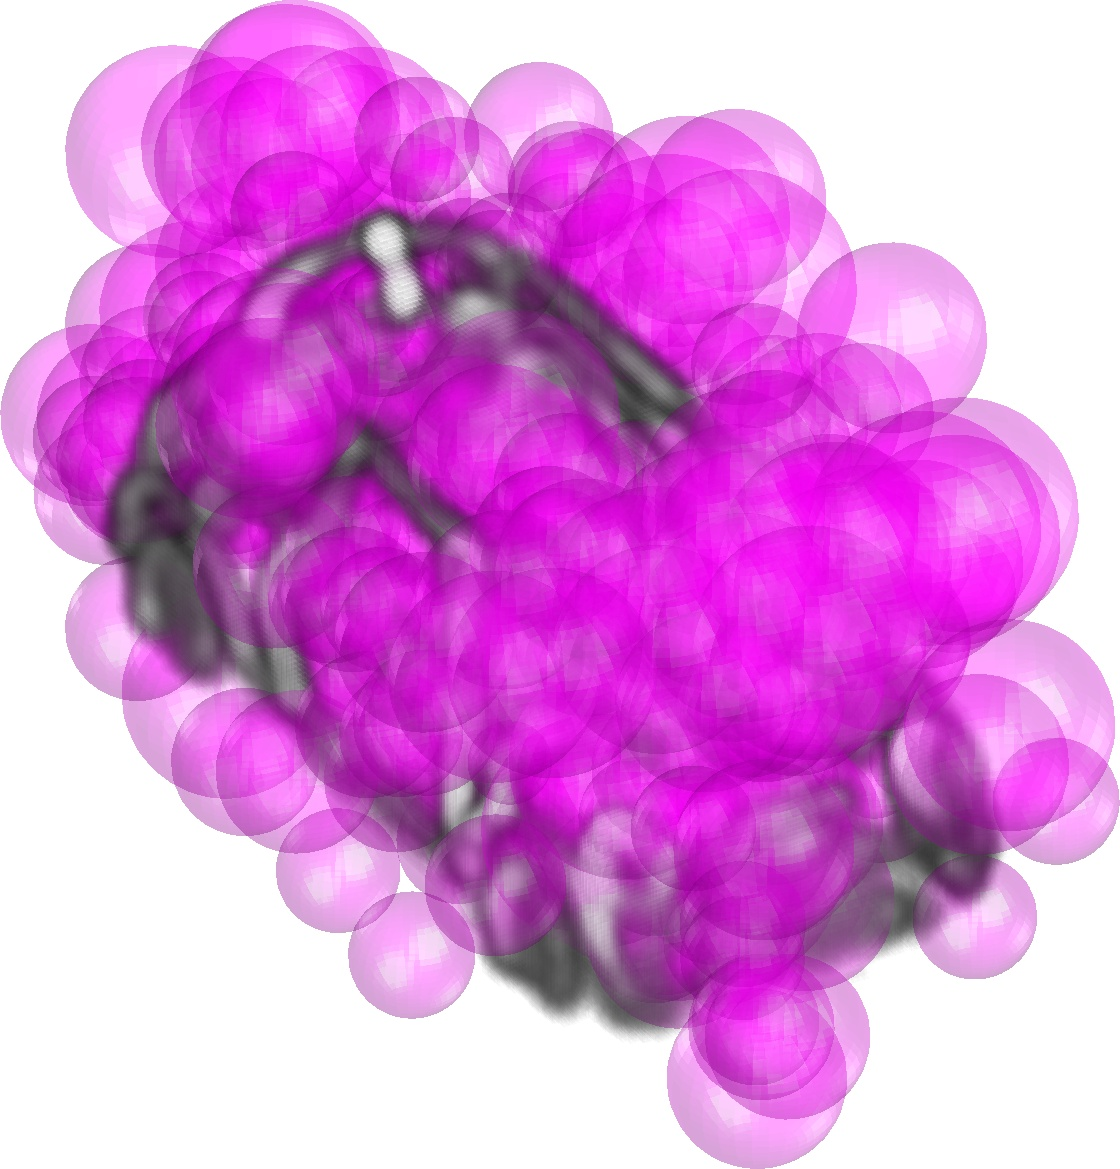
\includegraphics[width=0.180\linewidth]{./fig/eval/mini_surf.jpg} 
		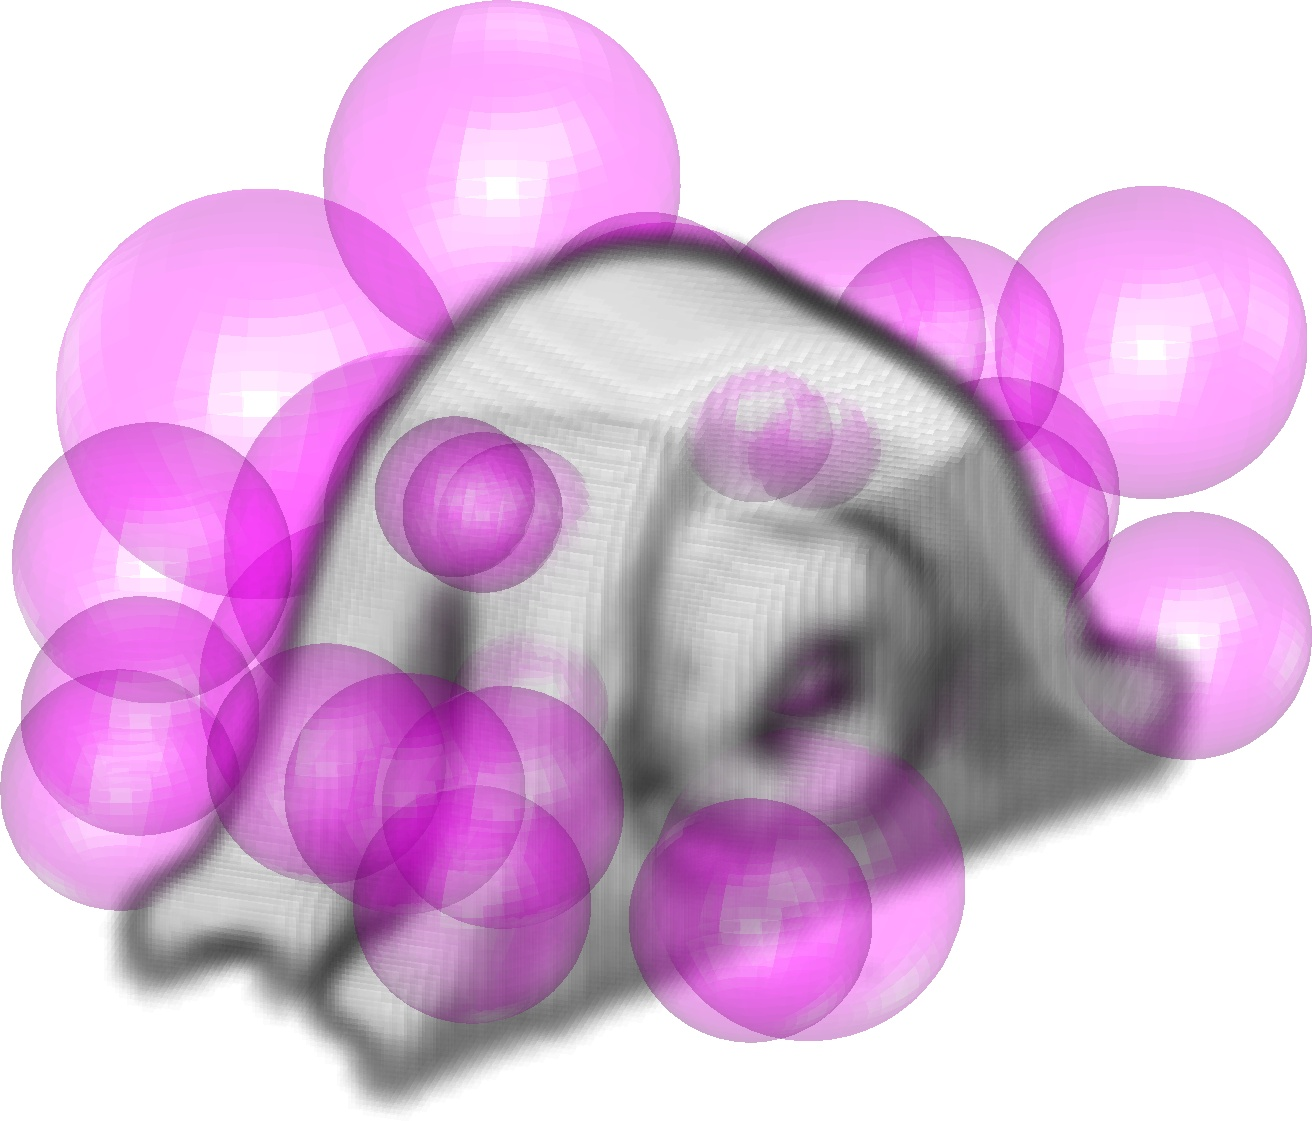
\includegraphics[width=0.180\linewidth]{./fig/eval/bearing_surf.jpg}  
		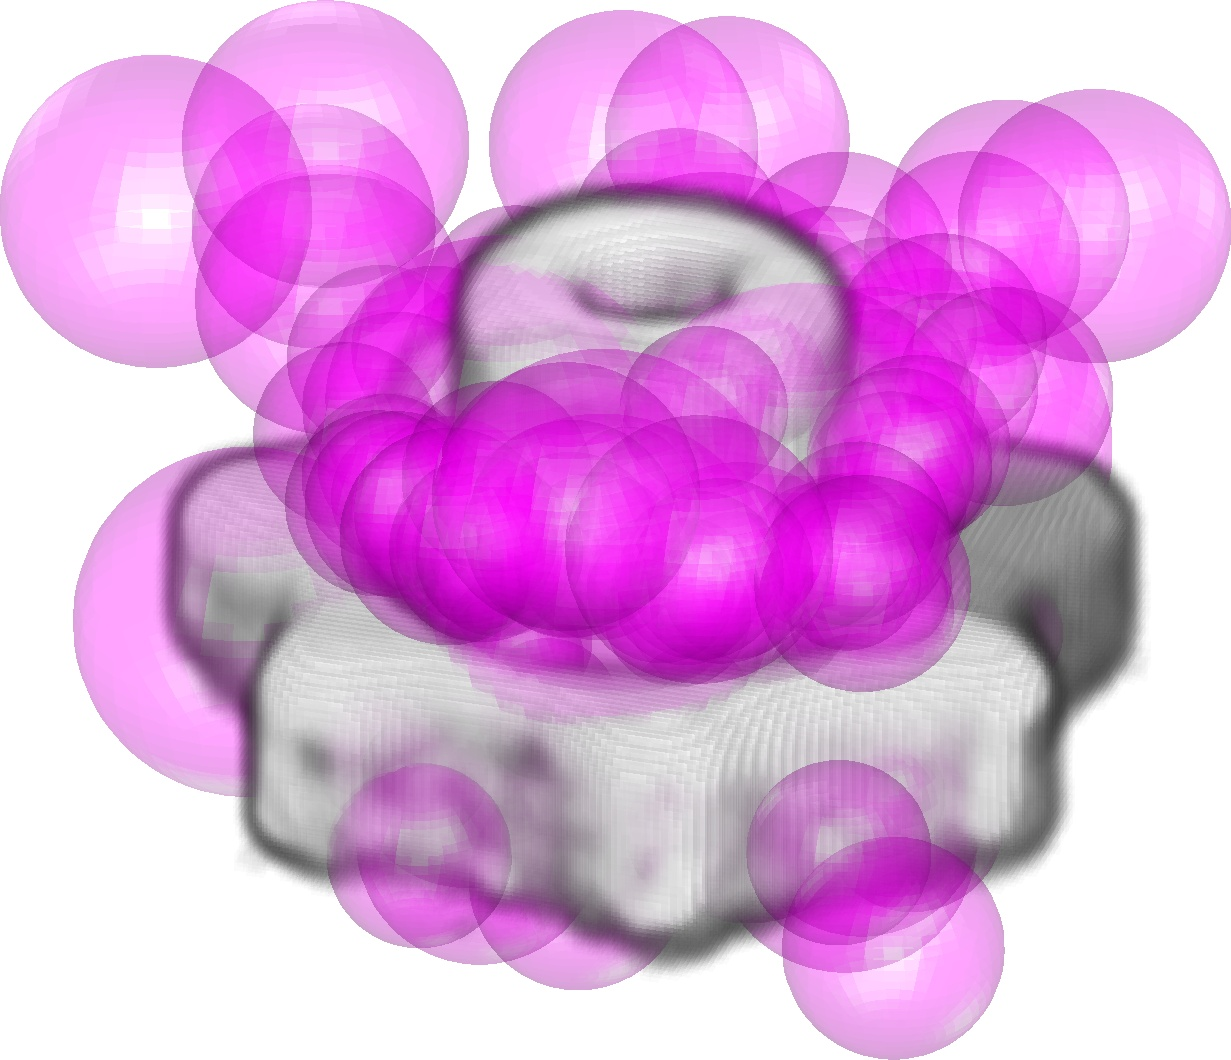
\includegraphics[width=0.180\linewidth]{./fig/eval/knob_surf.jpg} 
		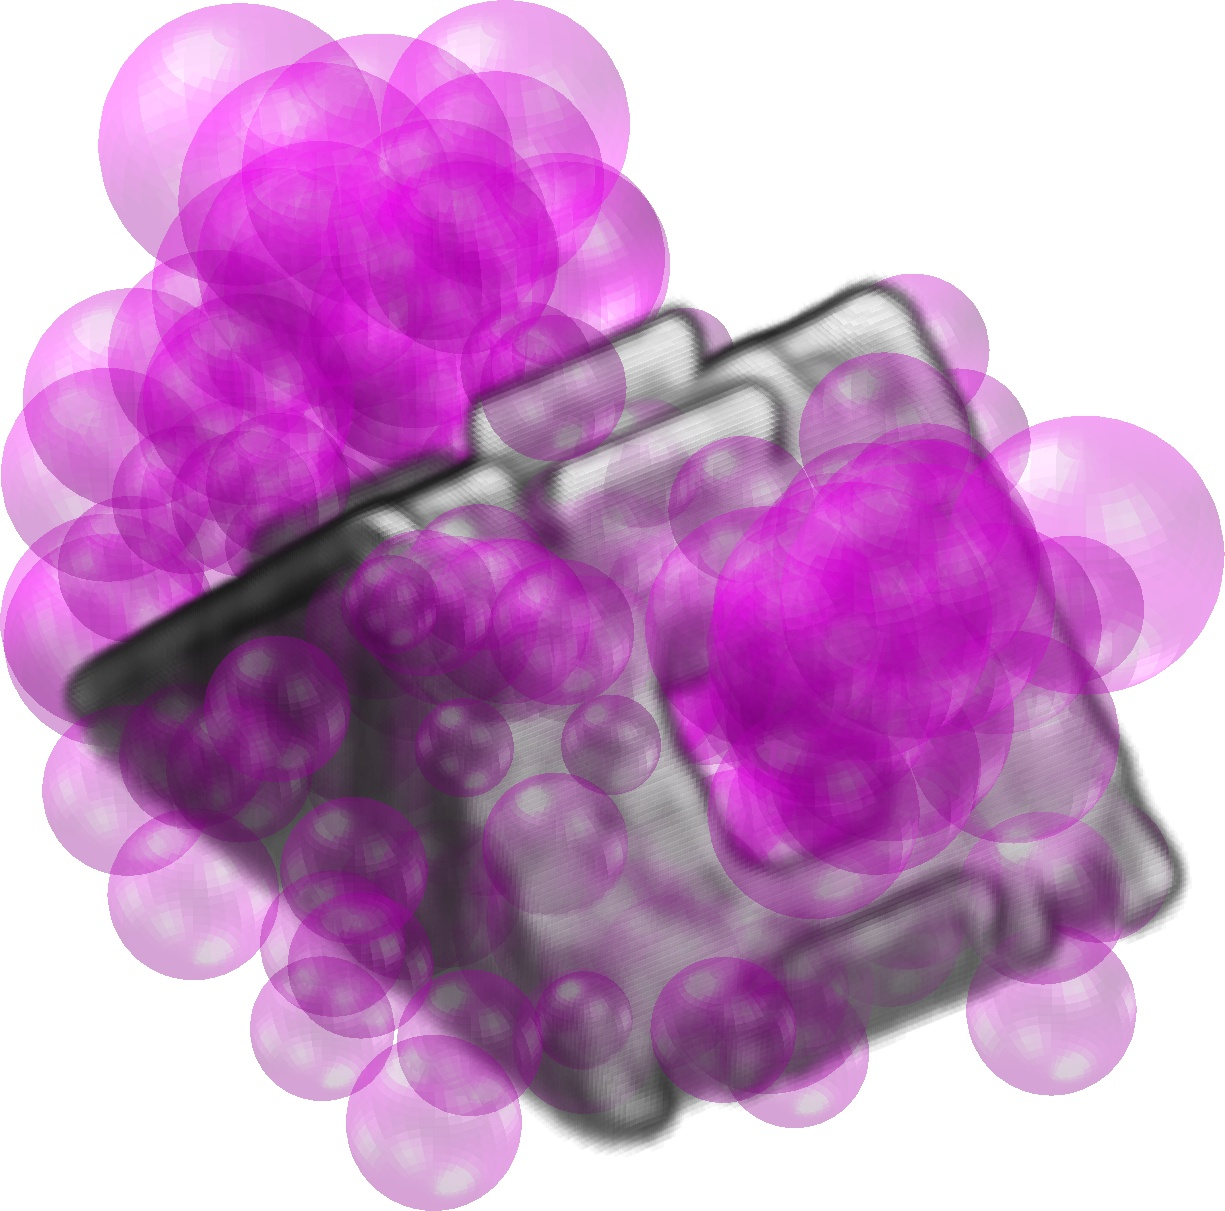
\includegraphics[width=0.180\linewidth]{./fig/eval/bracket_surf.jpg} 
	\end{subfigure}
	\begin{subfigure}[t]{1\linewidth} \centering
		\phantomcaption 
		\label{fig/eval/mvs/harris}
		\makebox[0.15\linewidth]{\raisebox{0.07\linewidth}{(d) Harris}}		
		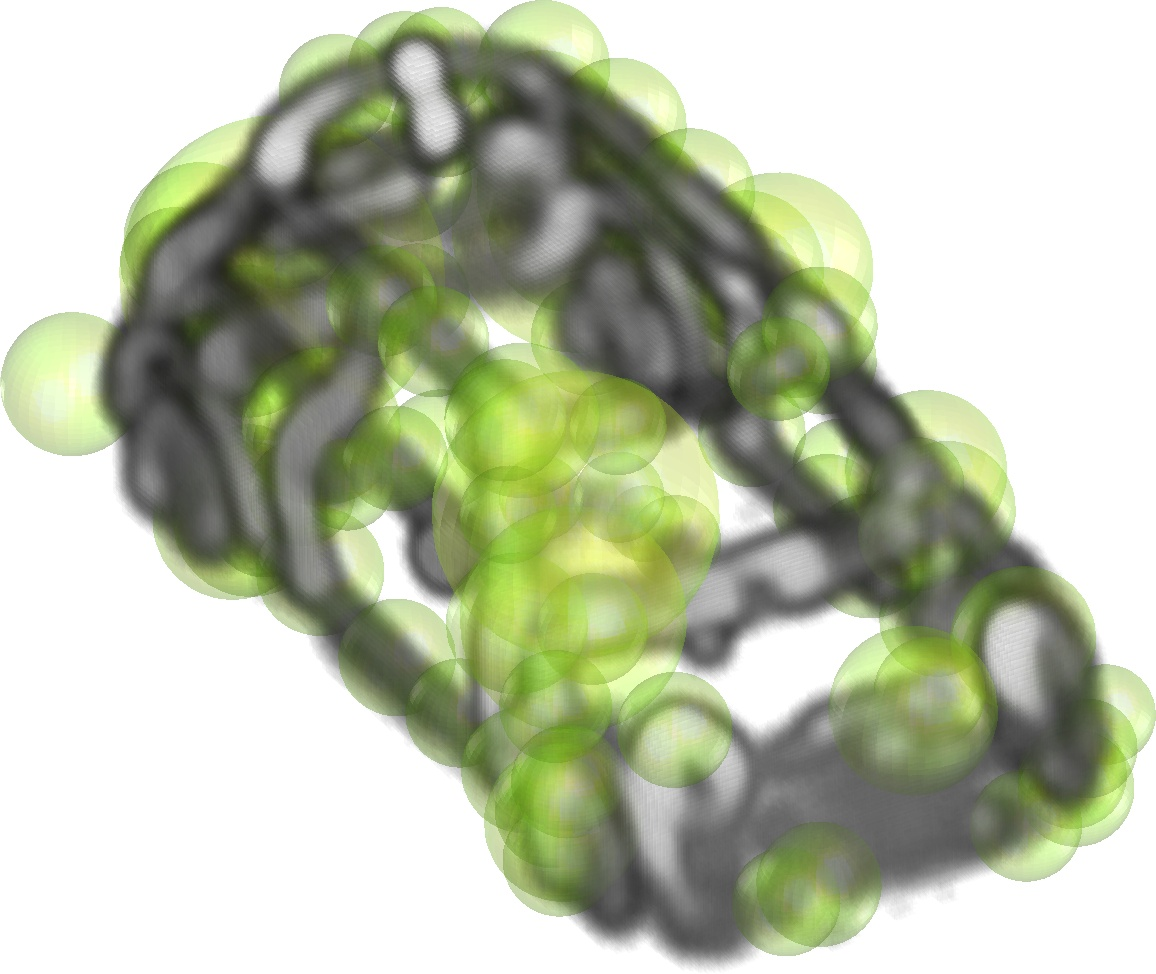
\includegraphics[width=0.180\linewidth]{./fig/eval/mini_harris.jpg} 
		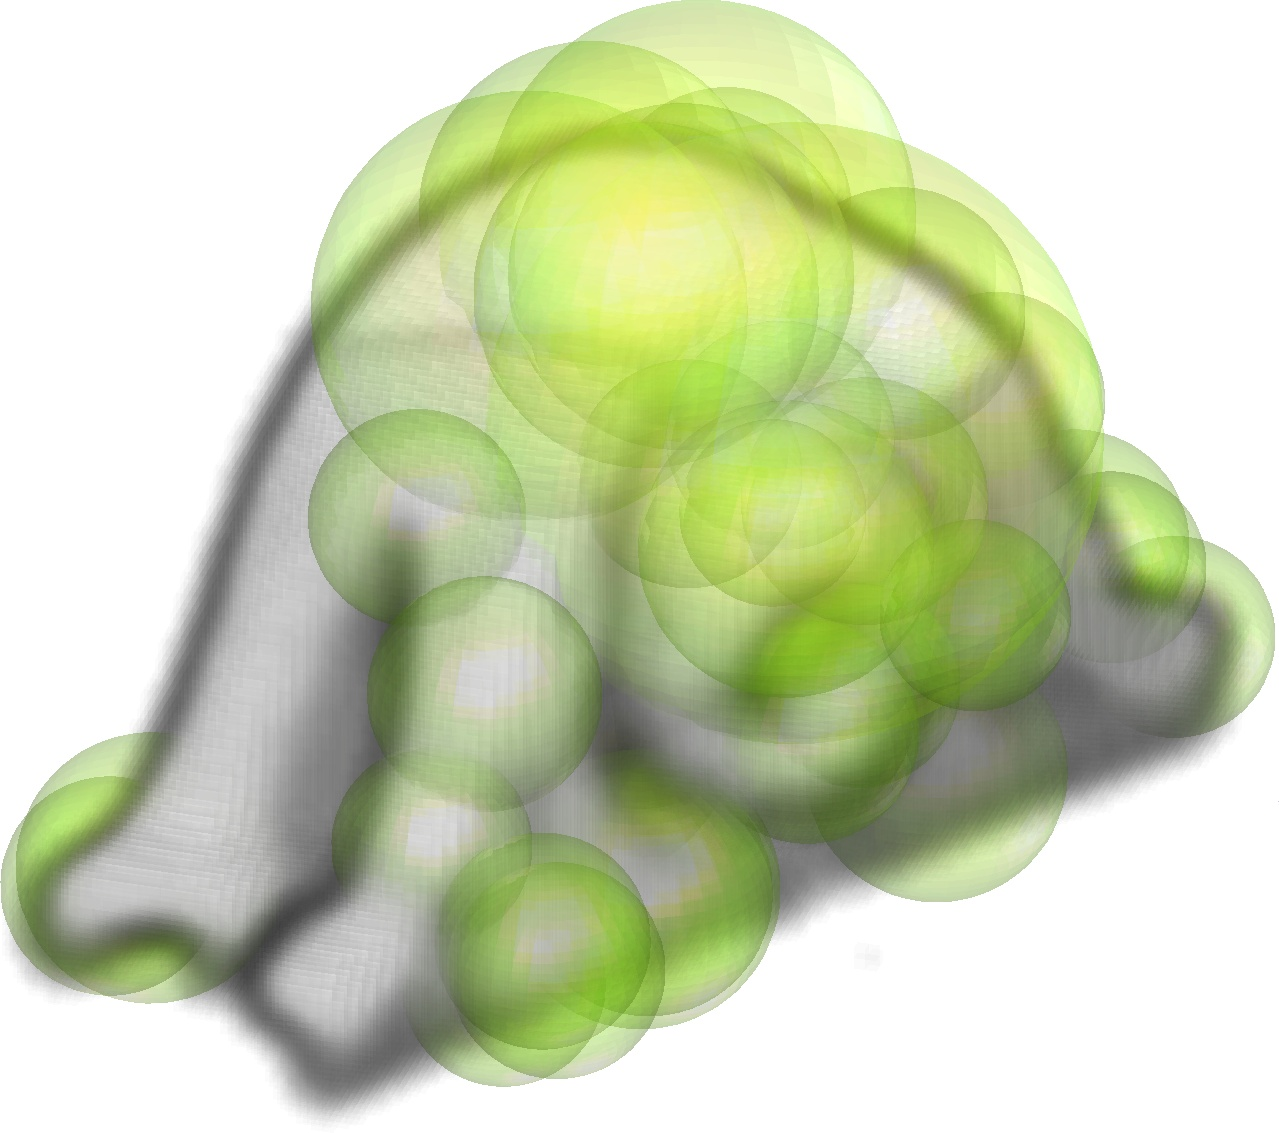
\includegraphics[width=0.180\linewidth]{./fig/eval/bearing_harris.jpg}  
		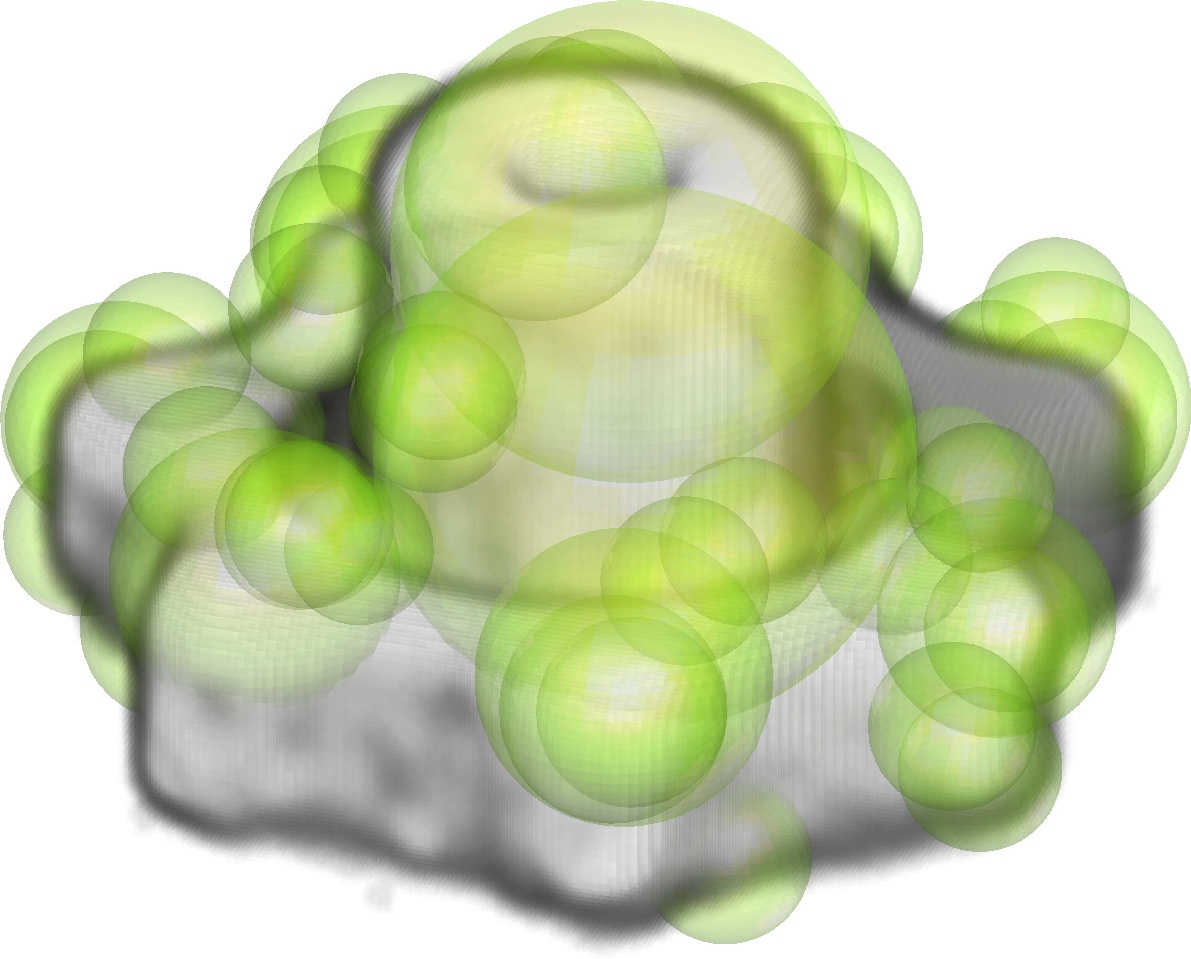
\includegraphics[width=0.180\linewidth]{./fig/eval/knob_harris.jpg} 
		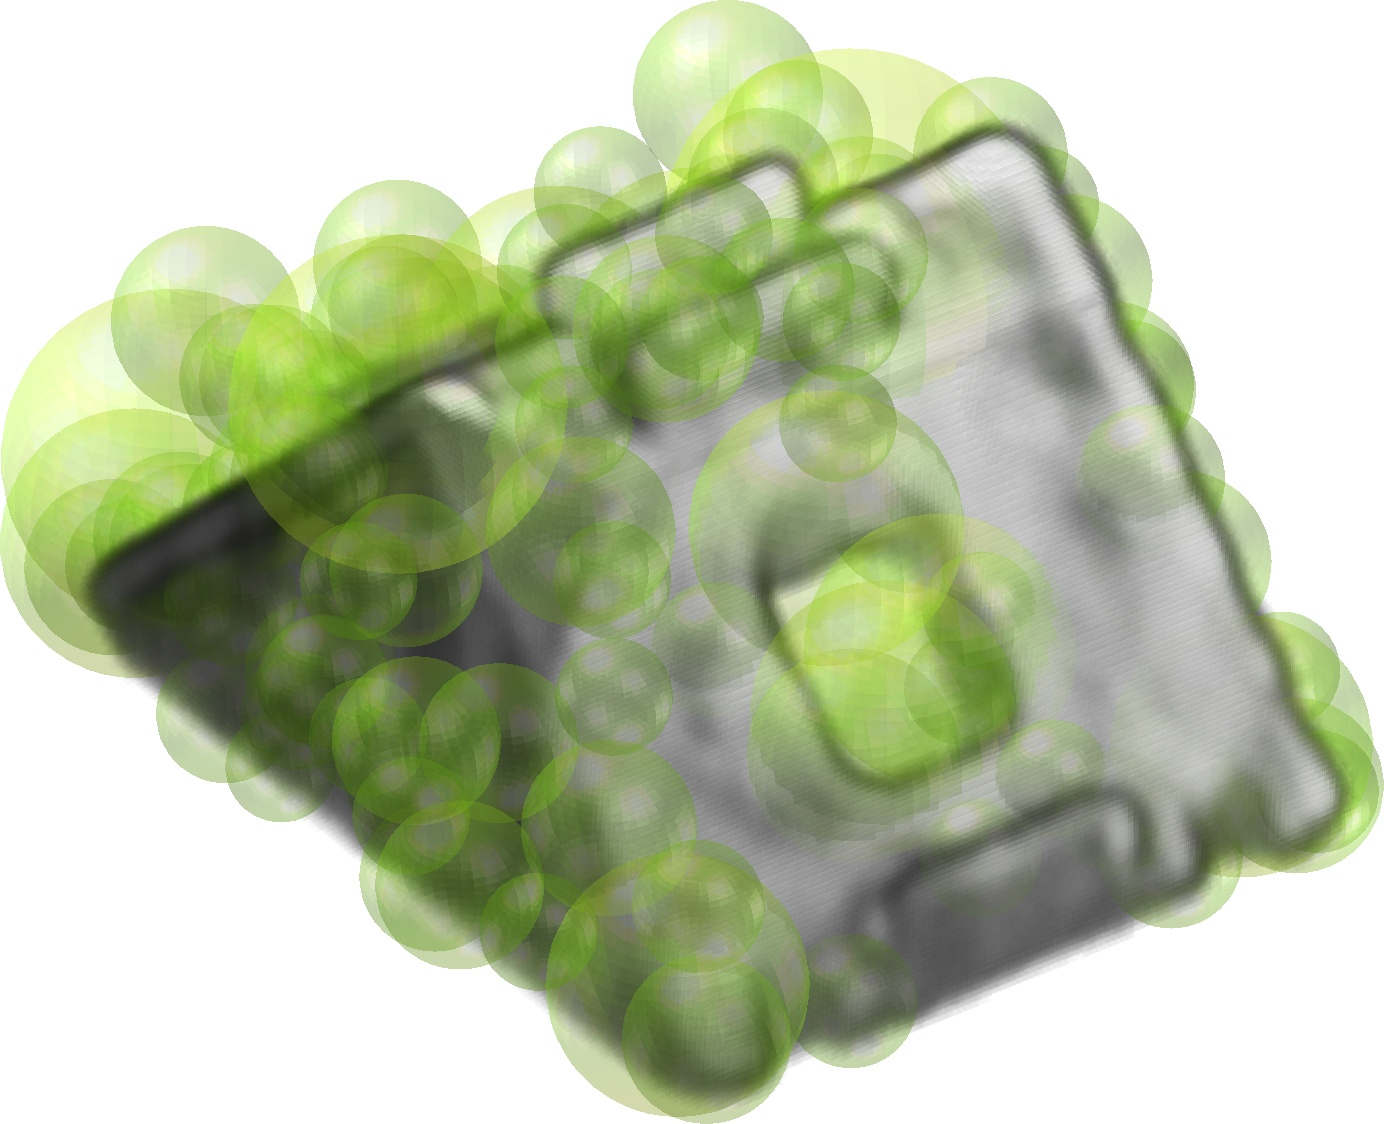
\includegraphics[width=0.180\linewidth]{./fig/eval/bracket_harris.jpg} 
	\end{subfigure}
	\begin{subfigure}[t]{1\linewidth} \centering
		\phantomcaption 
		\label{fig/eval/mvs/hessian}
		\makebox[0.15\linewidth]{\raisebox{0.07\linewidth}{(e) Hessian}}		
		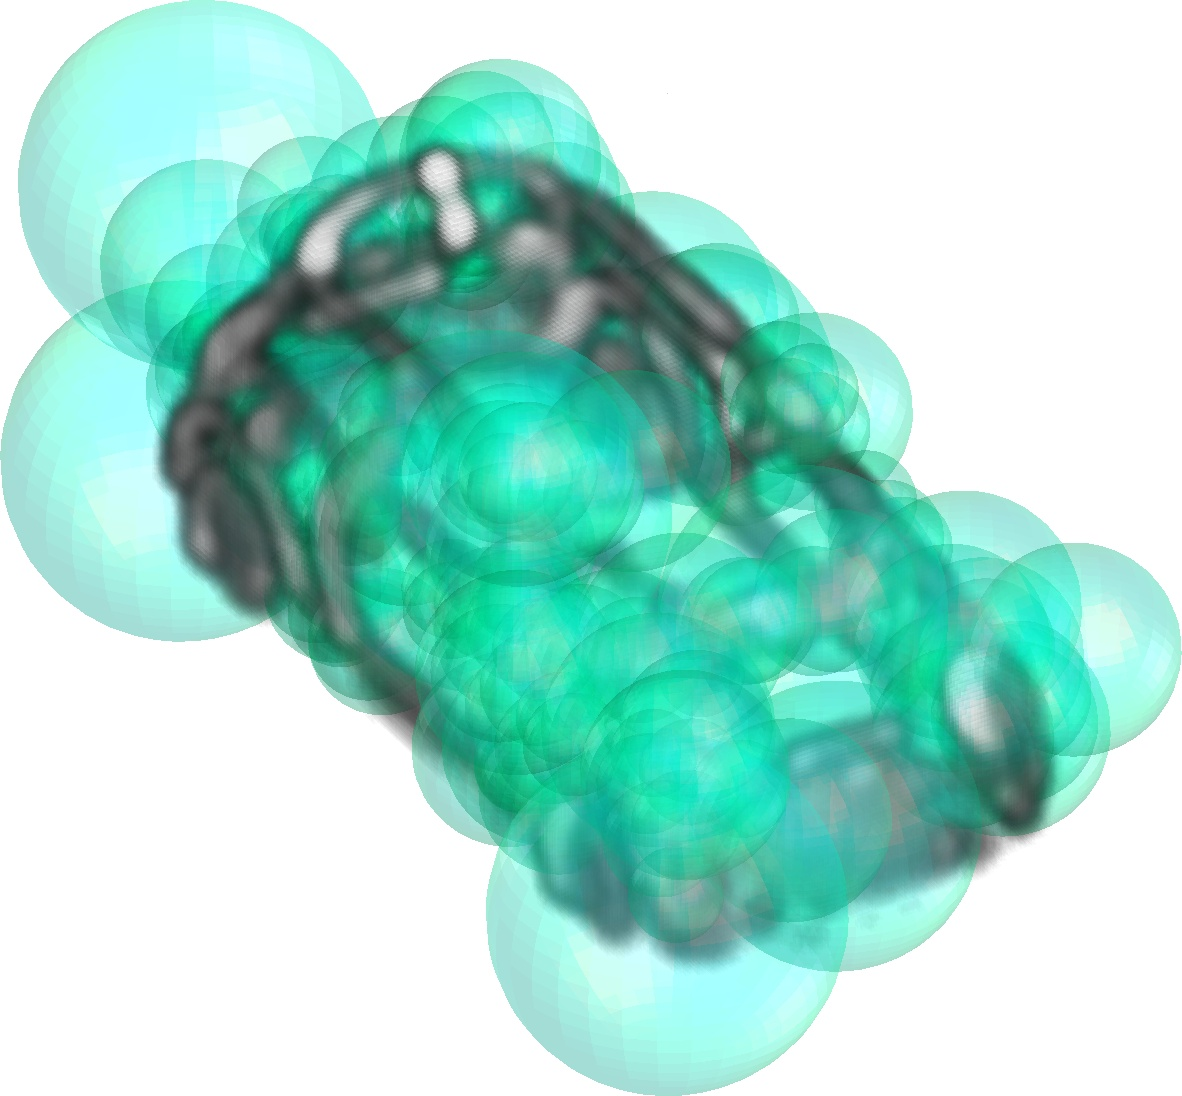
\includegraphics[width=0.180\linewidth]{./fig/eval/mini_hessian.jpg} 
		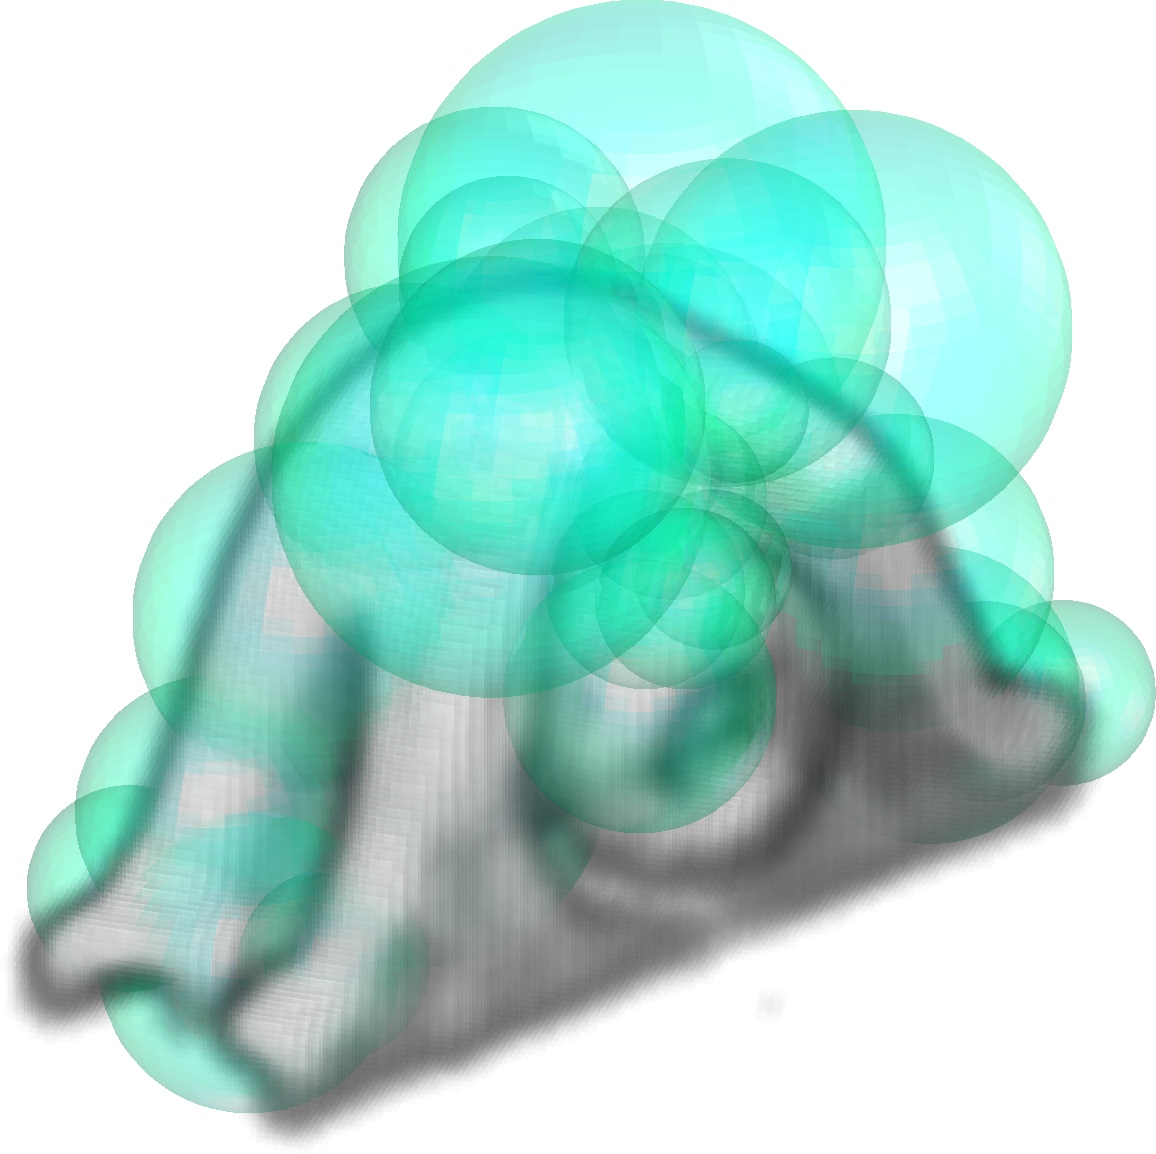
\includegraphics[width=0.180\linewidth]{./fig/eval/bearing_hessian.jpg}  
		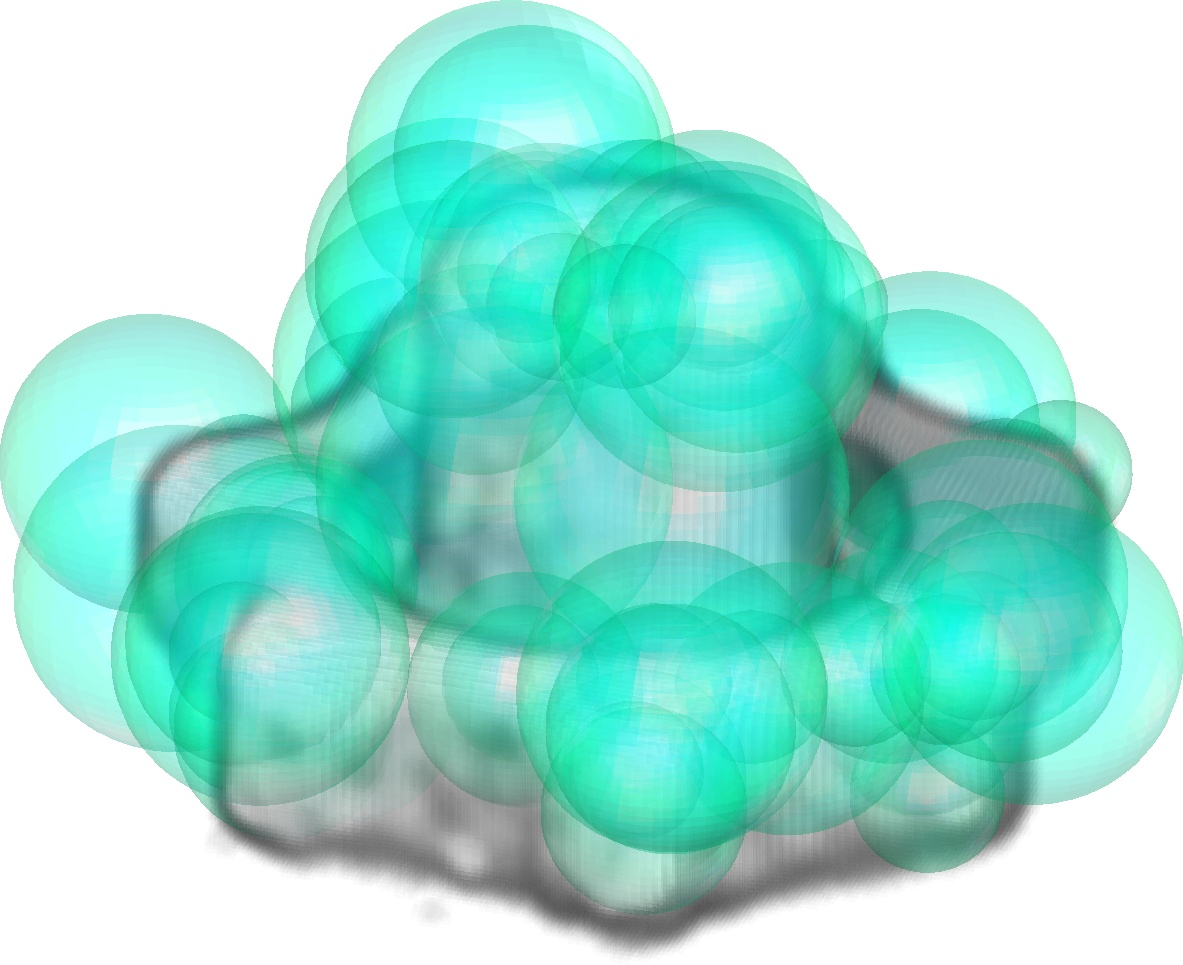
\includegraphics[width=0.180\linewidth]{./fig/eval/knob_hessian.jpg} 
		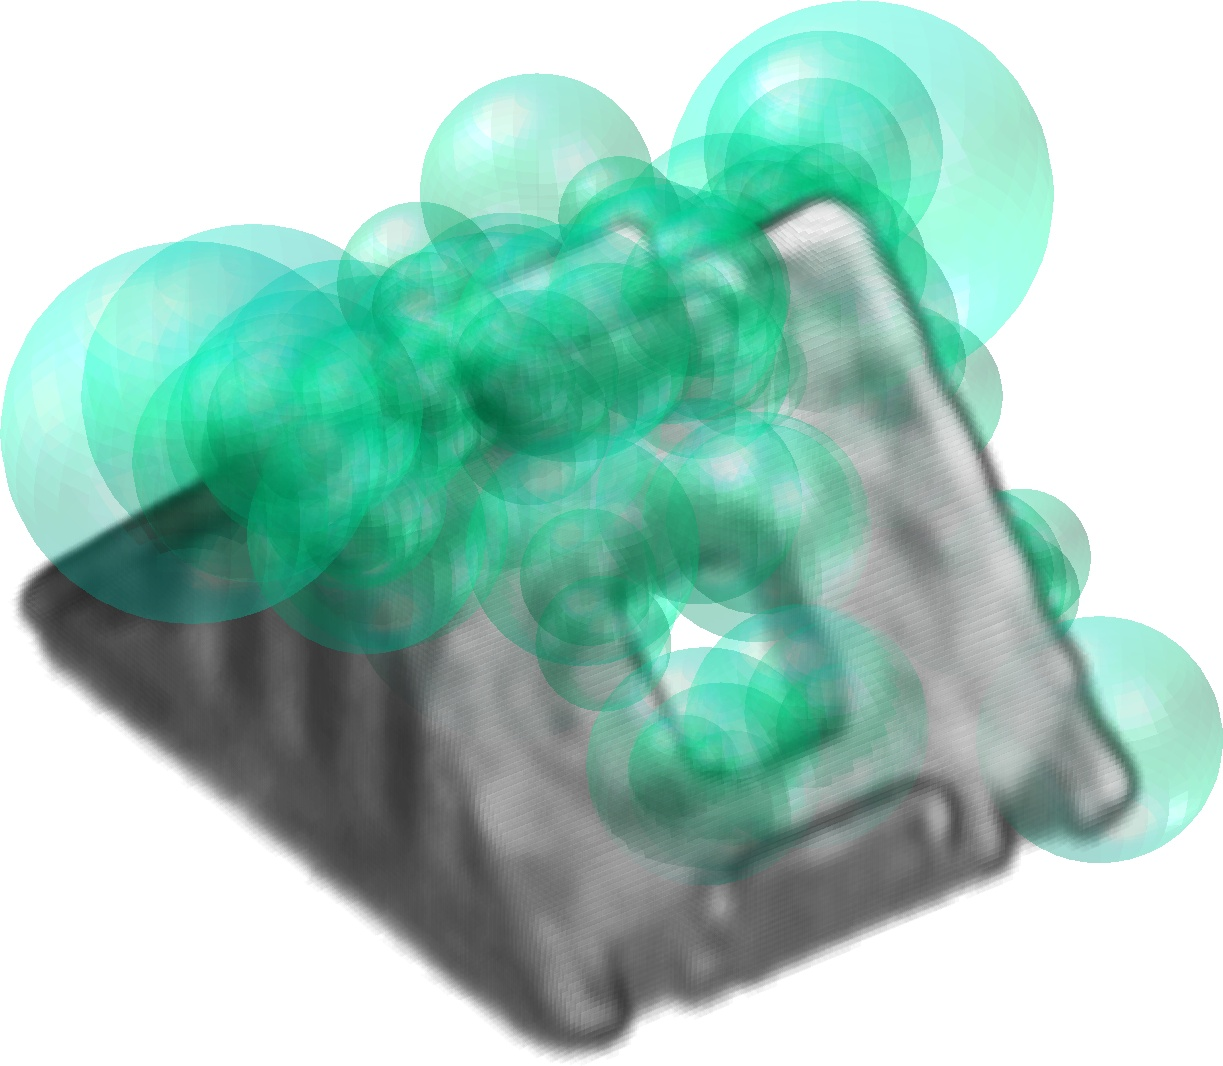
\includegraphics[width=0.180\linewidth]{./fig/eval/bracket_hessian.jpg} 
	\end{subfigure}
	\begin{subfigure}[t]{1\linewidth} \centering
		\phantomcaption 
		\label{fig/eval/mvs/vfast}
		\makebox[0.15\linewidth]{\raisebox{0.07\linewidth}{(f) VFAST}}		
		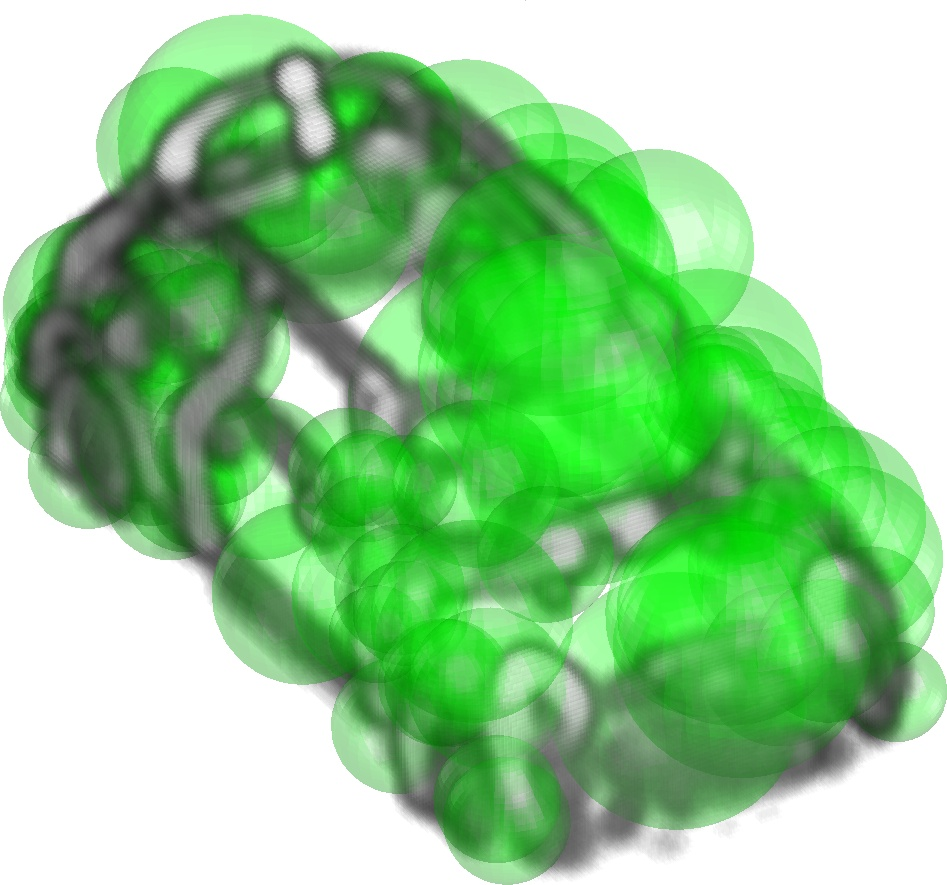
\includegraphics[width=0.180\linewidth]{./fig/eval/mini_fast.jpg} 
		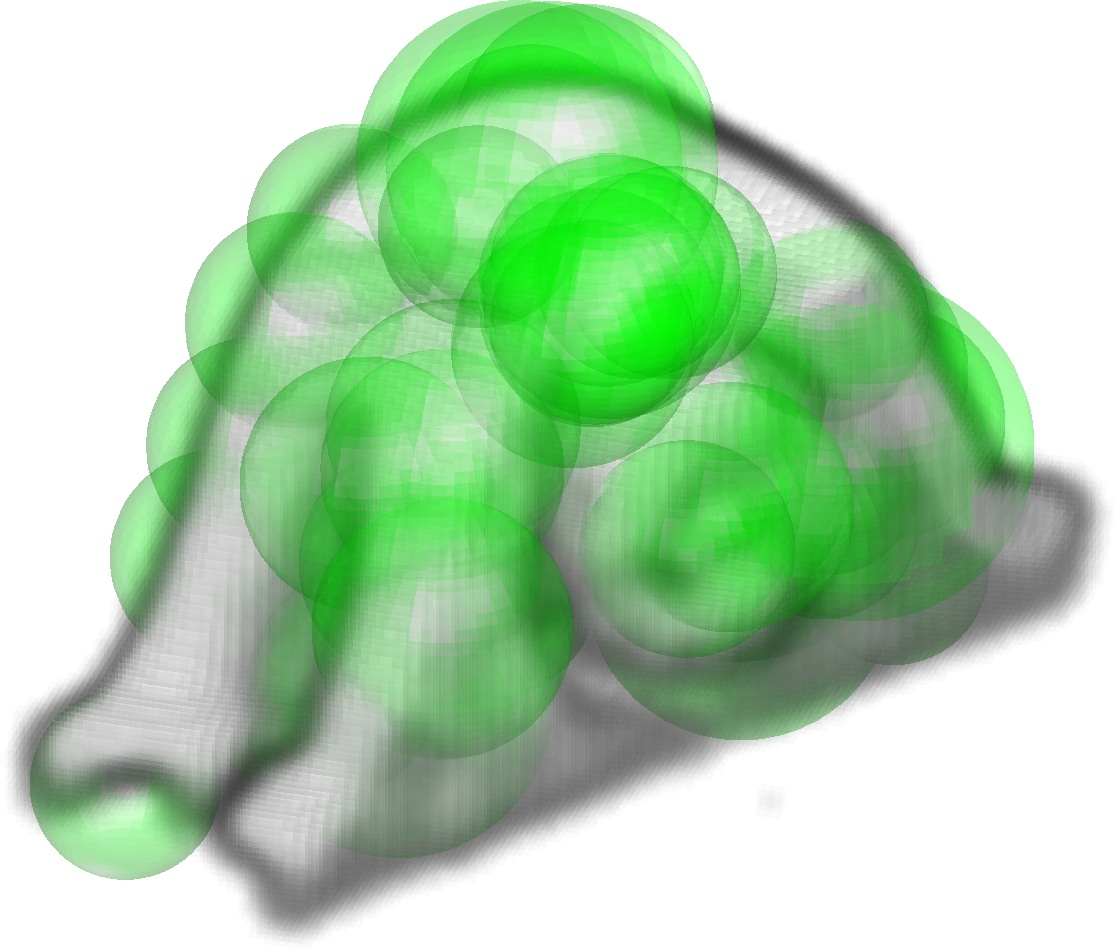
\includegraphics[width=0.180\linewidth]{./fig/eval/bearing_fast.jpg}  
		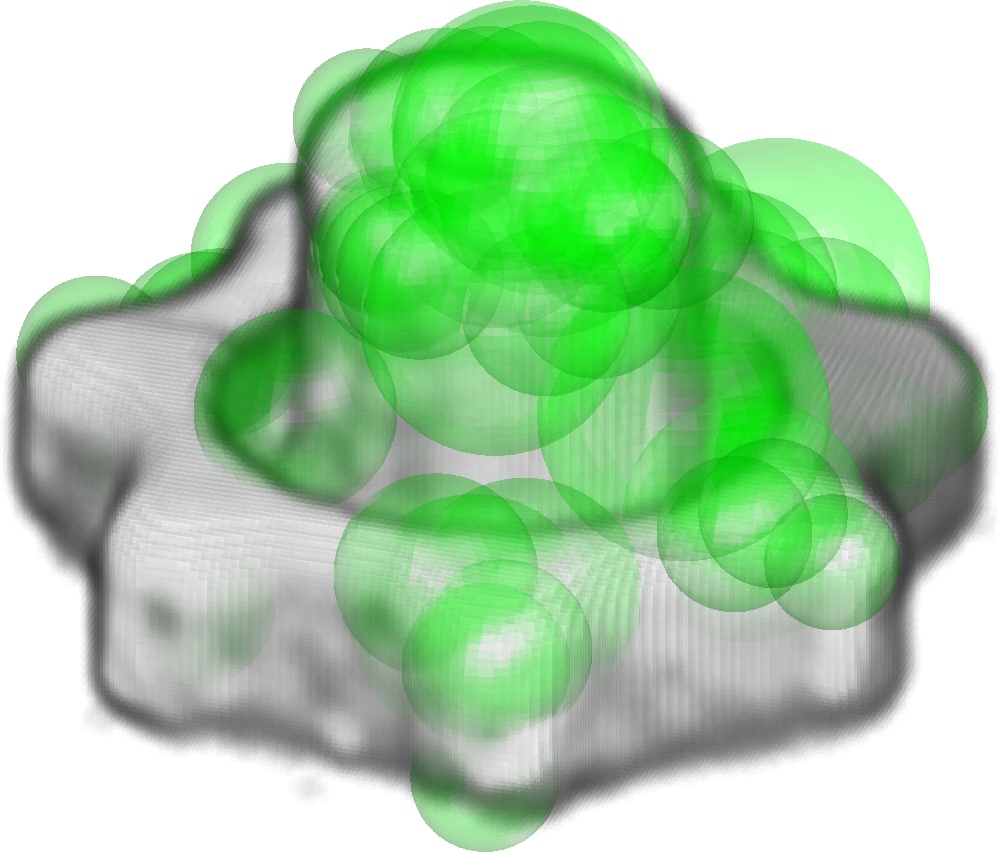
\includegraphics[width=0.180\linewidth]{./fig/eval/knob_fast.jpg} 
		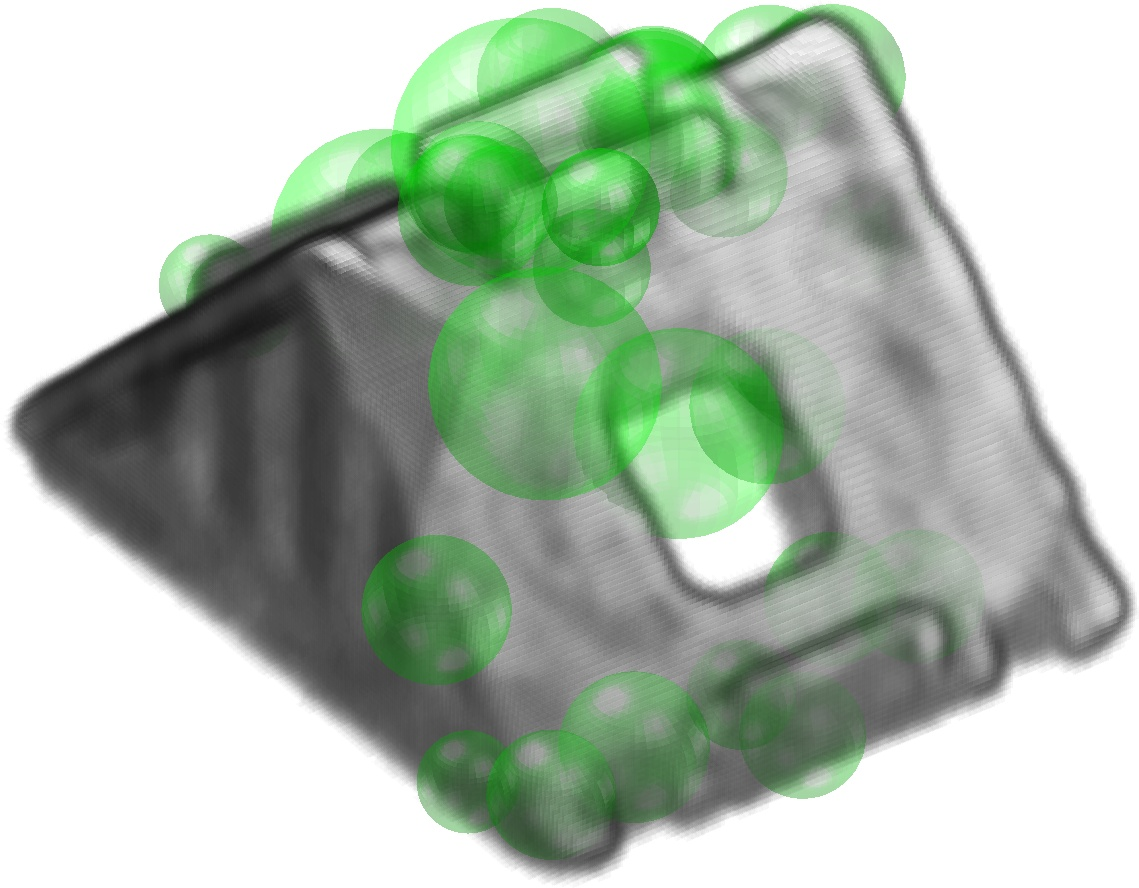
\includegraphics[width=0.180\linewidth]{./fig/eval/bracket_fast.jpg} 
	\end{subfigure}
	\begin{subfigure}[t]{1\linewidth} \centering
		\phantomcaption 
		\label{fig/eval/mvs/mser}
		\makebox[0.15\linewidth]{\raisebox{0.07\linewidth}{(g) MSER}}	
		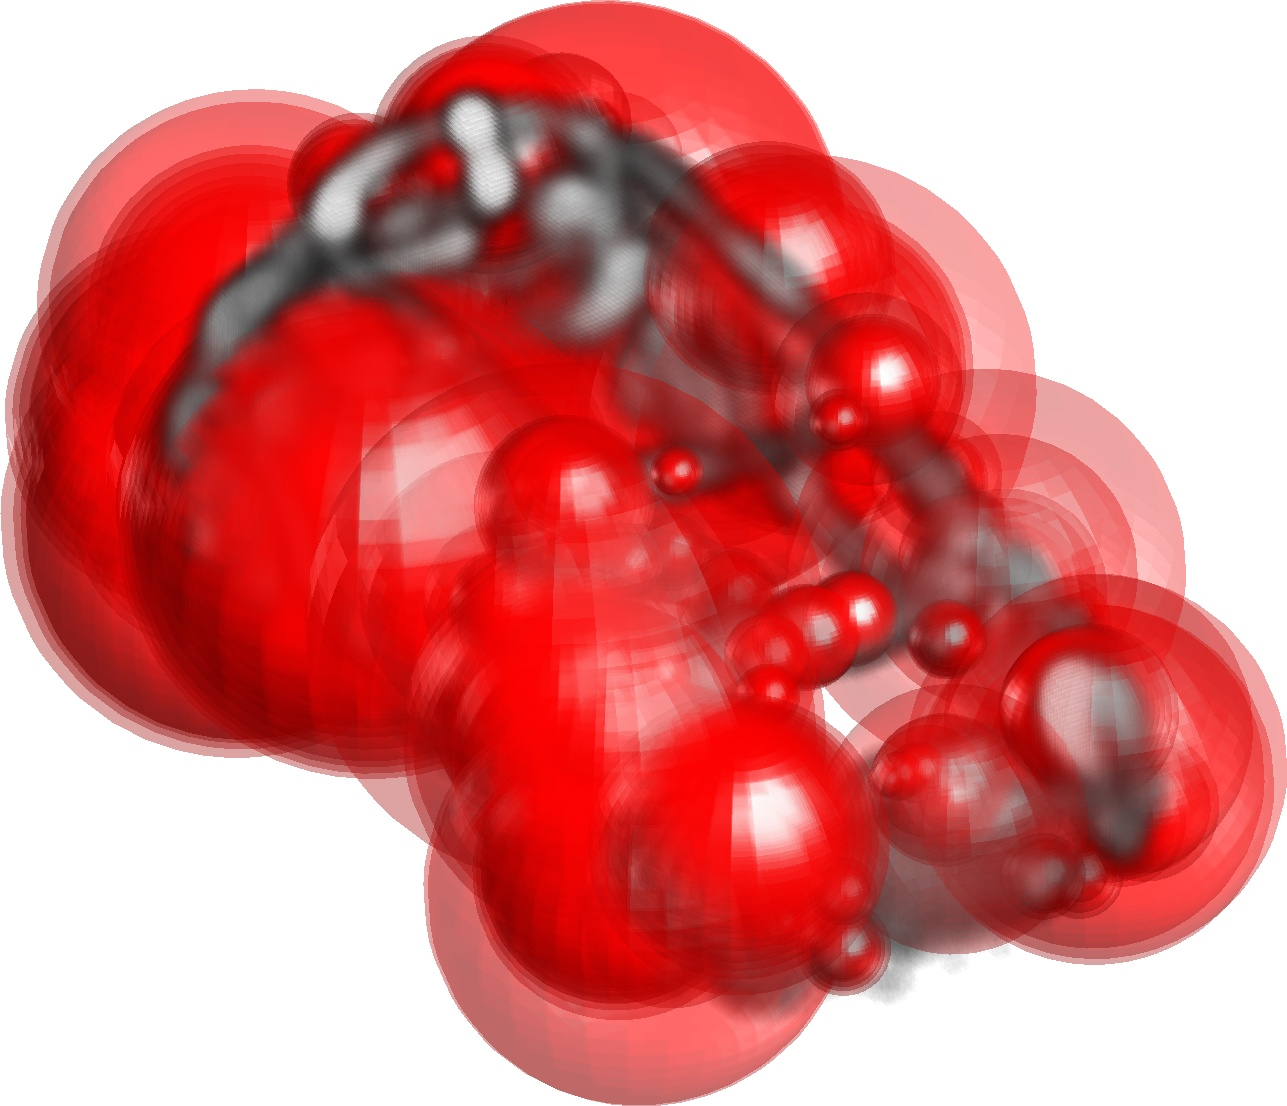
\includegraphics[width=0.180\linewidth]{./fig/eval/mini_mser.jpg} 
		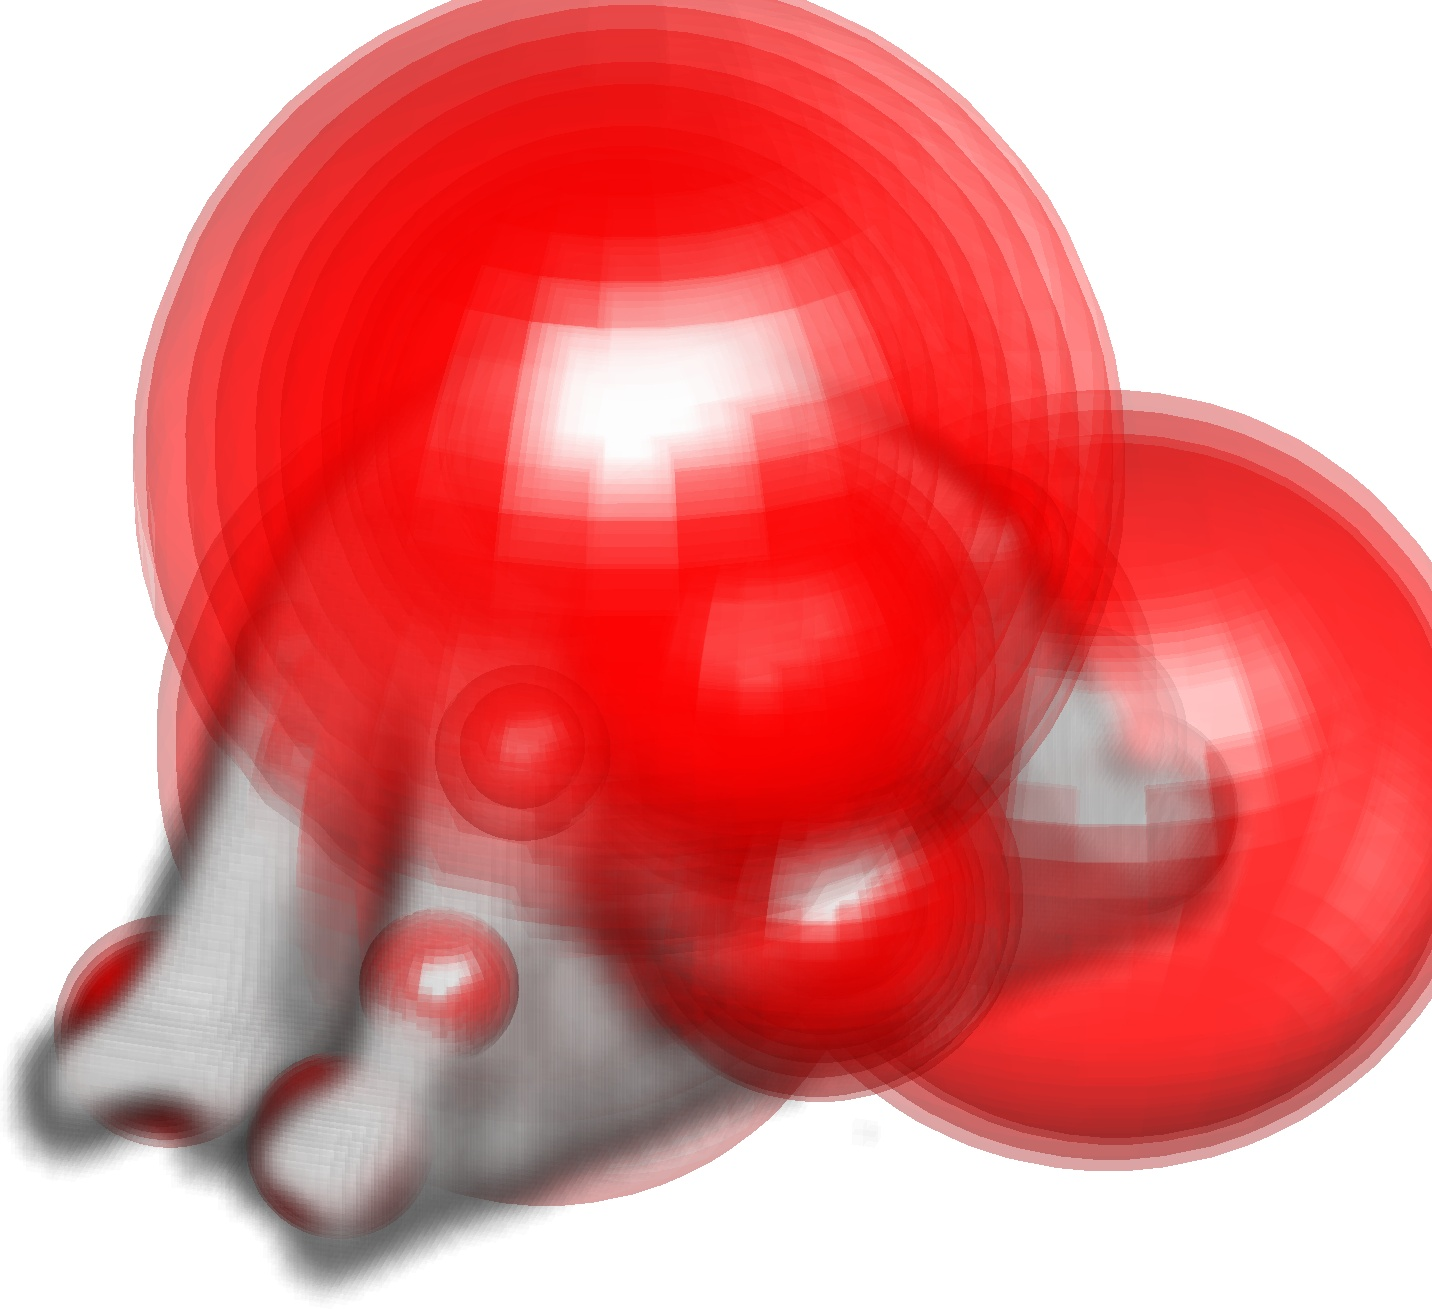
\includegraphics[width=0.180\linewidth]{./fig/eval/bearing_mser.jpg}  
		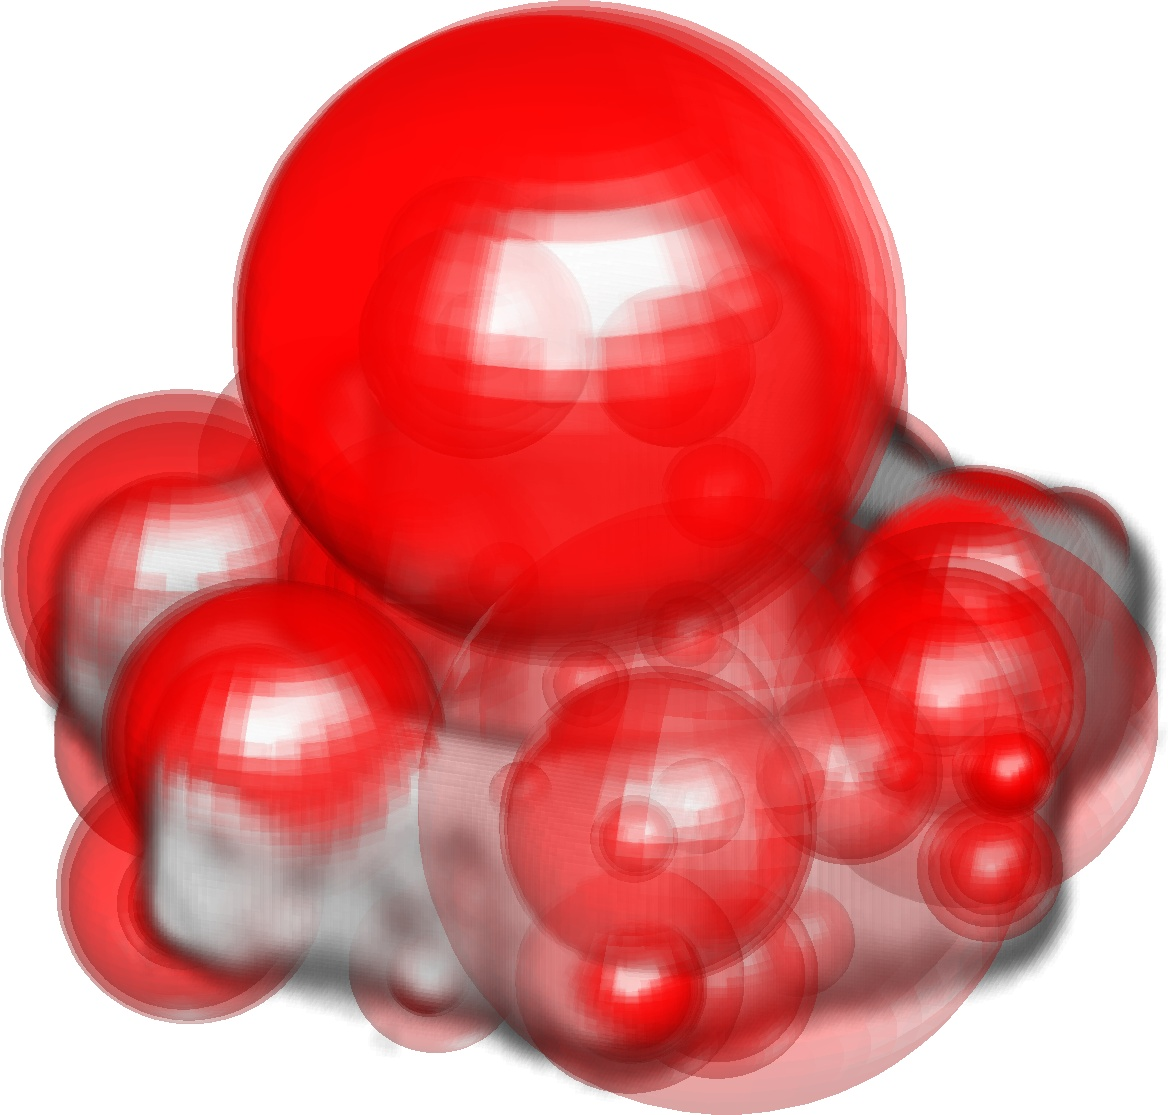
\includegraphics[width=0.180\linewidth]{./fig/eval/knob_mser.jpg} 
		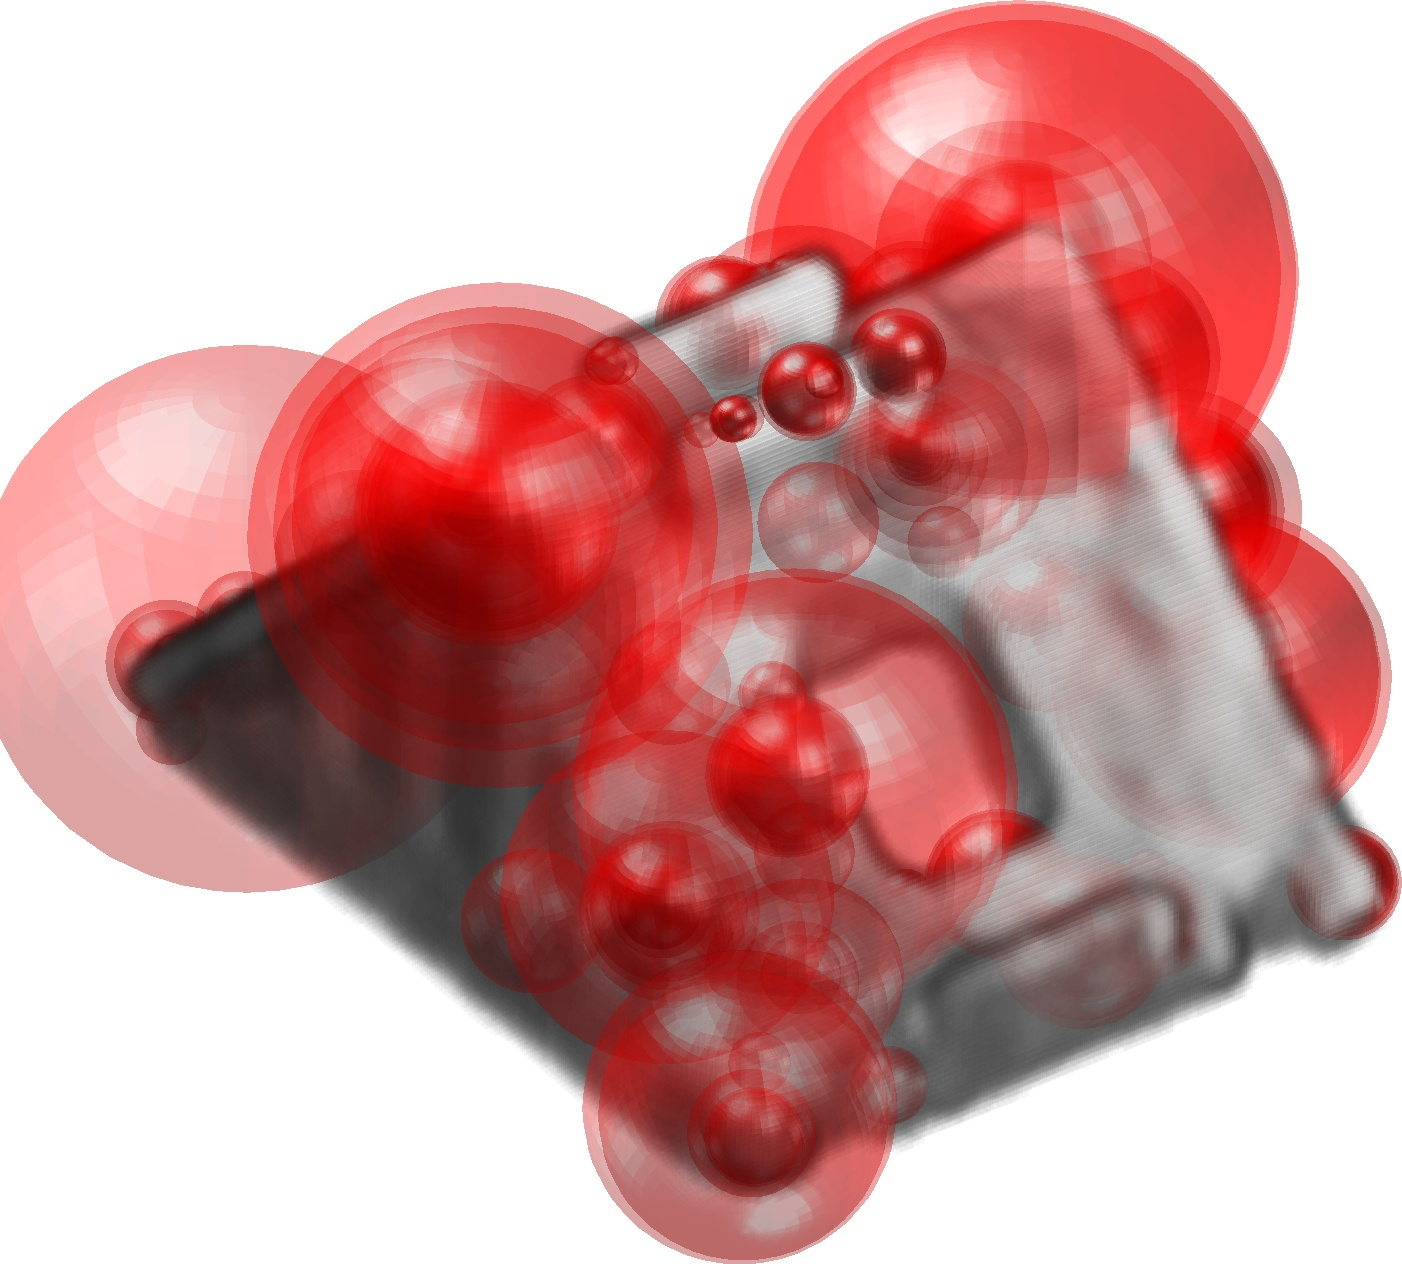
\includegraphics[width=0.180\linewidth]{./fig/eval/bracket_mser.jpg} 
	\end{subfigure}
	\caption{(a) Sample point clouds obtained from the stereo dataset. (b) DoG, (c) SURF (d) Harris, (e) DoH, (f) V-FAST and (g) MSER interest points visualized on the voxelized data.}
	\label{fig/eval/mvs}
\end{figure}

